% ----------------------------------------------------------------
% Report Class (This is a LaTeX2e document)  *********************
% ----------------------------------------------------------------
% Dissertation Template

\documentclass[11pt,oneside]{book}
% \usepackage[margin=1.2in]{geometry}
\usepackage[toc,page]{appendix}
\usepackage{graphicx}
%\usepackage{natbib}
\usepackage{lipsum}
\usepackage{caption}
\usepackage[numbers]{natbib}

%\documentclass[12pt,a4paper]{report}

\usepackage[lmargin=2.54cm,tmargin=1cm,rmargin=2.54cm,bmargin=1cm]{geometry}
\usepackage{mathptmx}

\begin{document}
\setcounter{tocdepth}{0} 
\renewcommand\labelitemi{---}

\frontmatter

\begin{titlepage}
\begin{center}
{\LARGE University of Sheffield}\\[1.5cm]
\linespread{1.2}\Large {\bfseries EEE339}\\[2cm]
\linespread{1}

\includegraphics[width=9cm]{images/logo.png}\\[1.5cm]

\linespread{1.2}\Large {\bfseries Digital Signal Processing Coursework}\\[1cm]
{\Large Mohammed Ayman Shaikh}\\[1cm]
\large A report submitted in fulfillment of the module\\EEE339 Digital Engineering\\[0.3cm] 
\textit{in the}\\[0.3cm]
School of Electronic and Electrical Engineering\\[2cm]
\today
\end{center}

\end{titlepage}


\linespread{1.5}

% Fonts -- the following two packages give you Times Roman in LaTex
%\usepackage{txfonts}


\pagenumbering{arabic}


\chapter{Introduction}
In this coursework, digital filters will be implemented in MATLAB to remove noise from 
Electrocardiogram (ECG) signals. The file \textbf{ECGData1.mat} will be used for the purposes of this coursework. The diagnosis for this data set was premature ventricular contraction (PVC), in a 69 year-old male
\chapter{Original and Noisy ECG Signals}
Below, two plots can be seen. 
\\The first plot is the original ECG signal, and the second is the same signal, but with added noise.
\begin{center}
%\centering
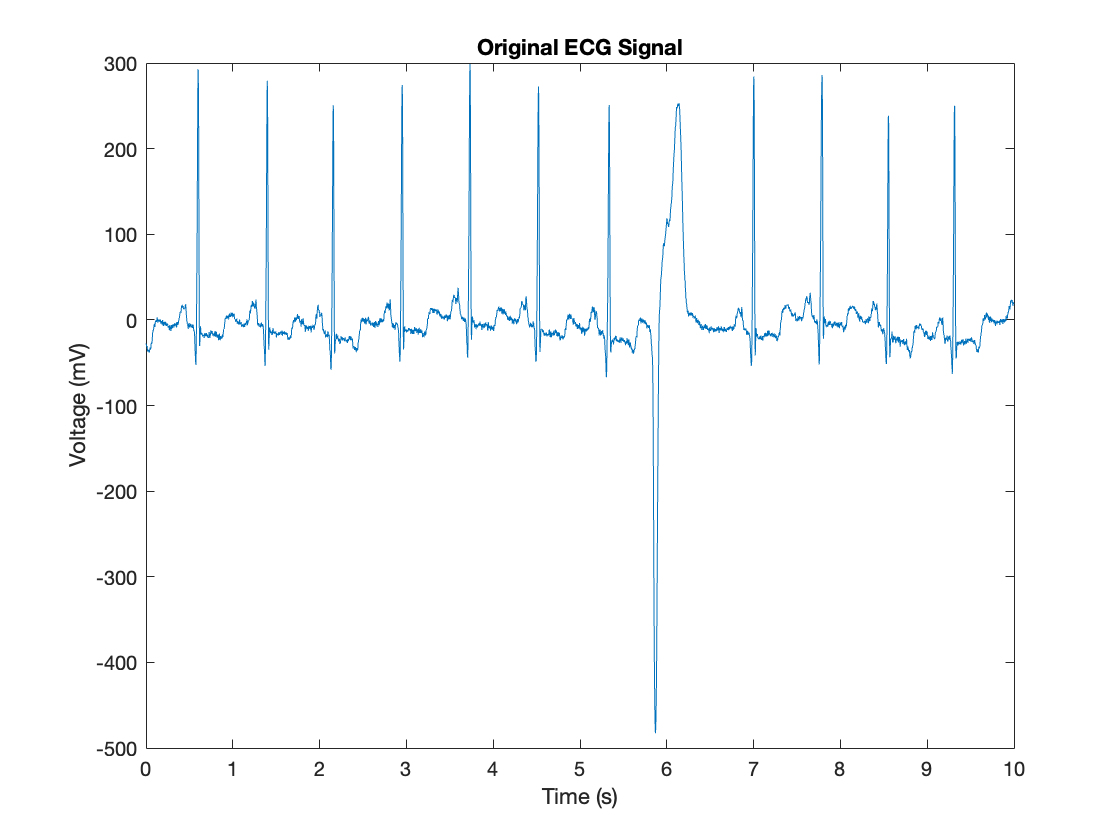
\includegraphics[width=10cm]{graphics/orig.png}
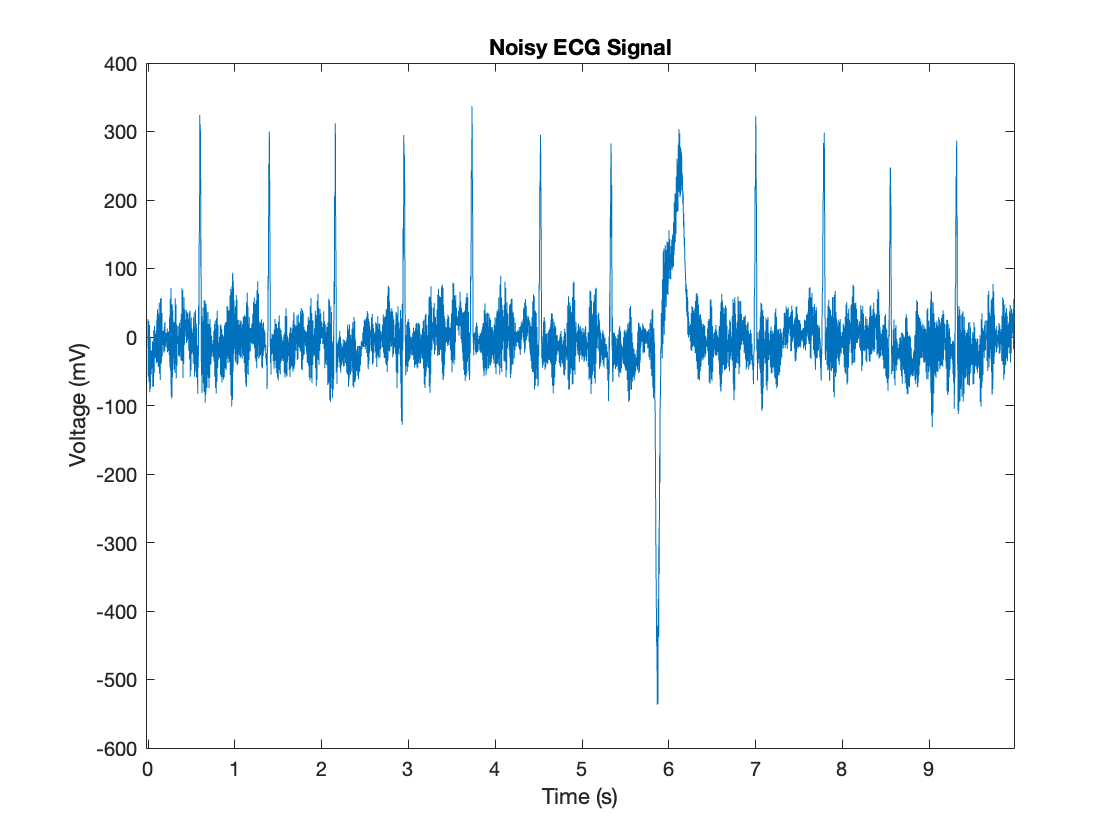
\includegraphics[width=10cm]{graphics/noisy.png}
\end{center}
\chapter{Heart Rate Calculation}
The heart rate can be calculated using the number of R-peaks in the ECG signals and knowledge of the timeframe of the signal recorded.
Since 12 R-peaks can be seen in both signals and the timeframe of the recorded signals is 10 seconds, we use this formula to calculate the heart rate in beats per minute (bpm):
\begin{center}
    $\textit{Heart Rate} = \frac{\textit{Number of R-peaks}}{\textit{Timeframe}} \times 60 = \frac{12}{10} \times 60 = 72$ bpm
\end{center}
\end{document}
% ----------------------------------------------------------------

